\begin{frame}{Memory consumption}

  \begin{columns}
    \begin{column}{0.5\textwidth}

      \only<1>{\includegraphics[width=\textwidth]{figures/memmf}}%
      \only<2>{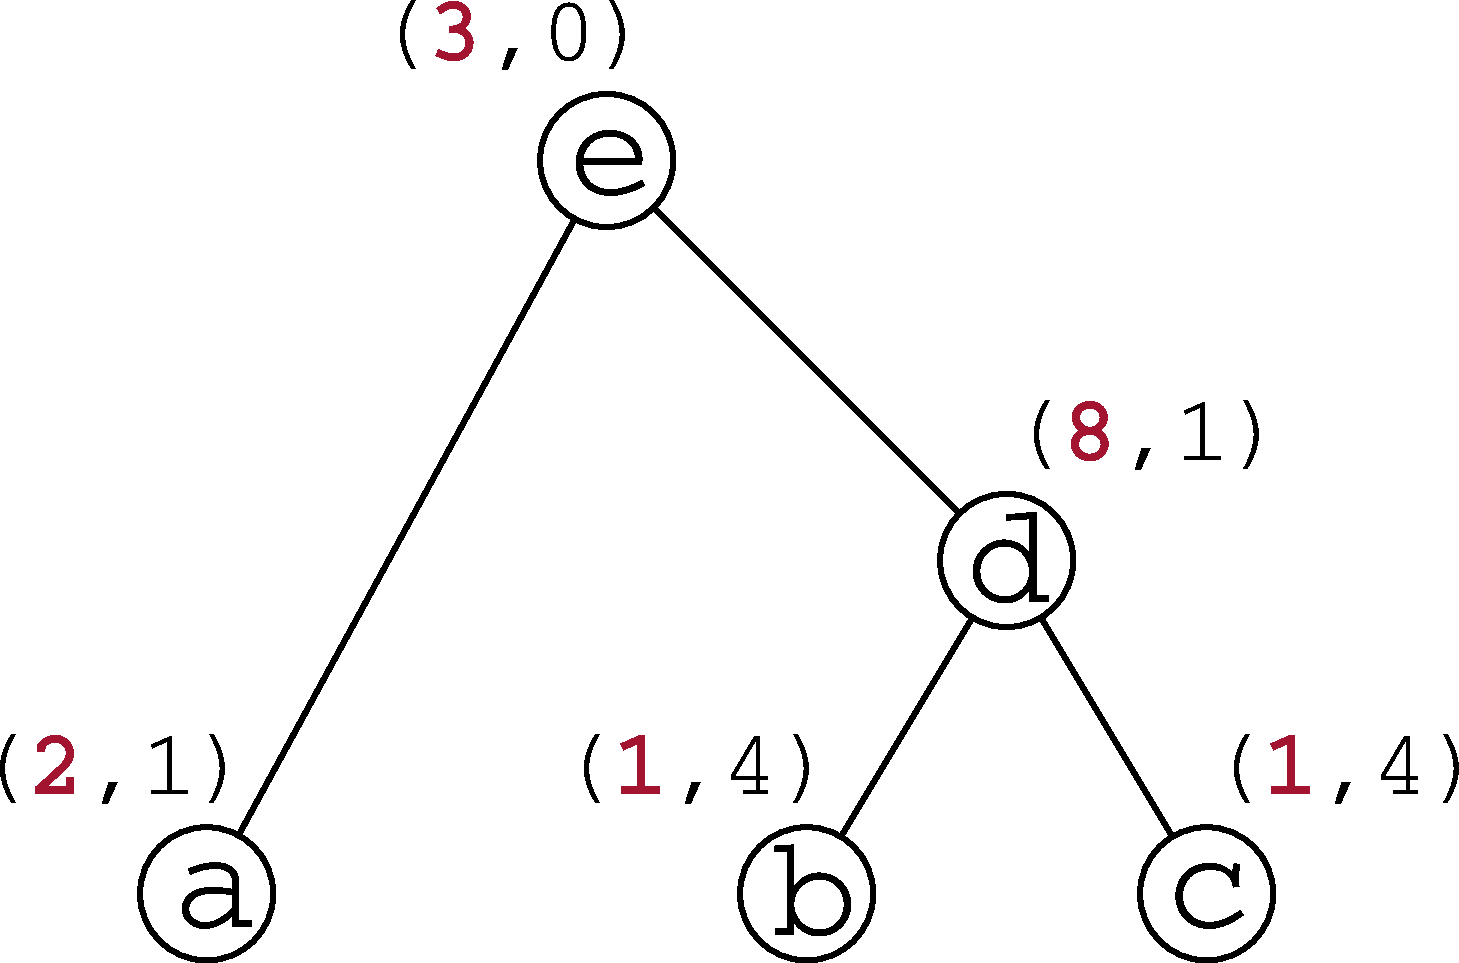
\includegraphics[width=\textwidth]{figures/memmf_factors}}%
      \only<3>{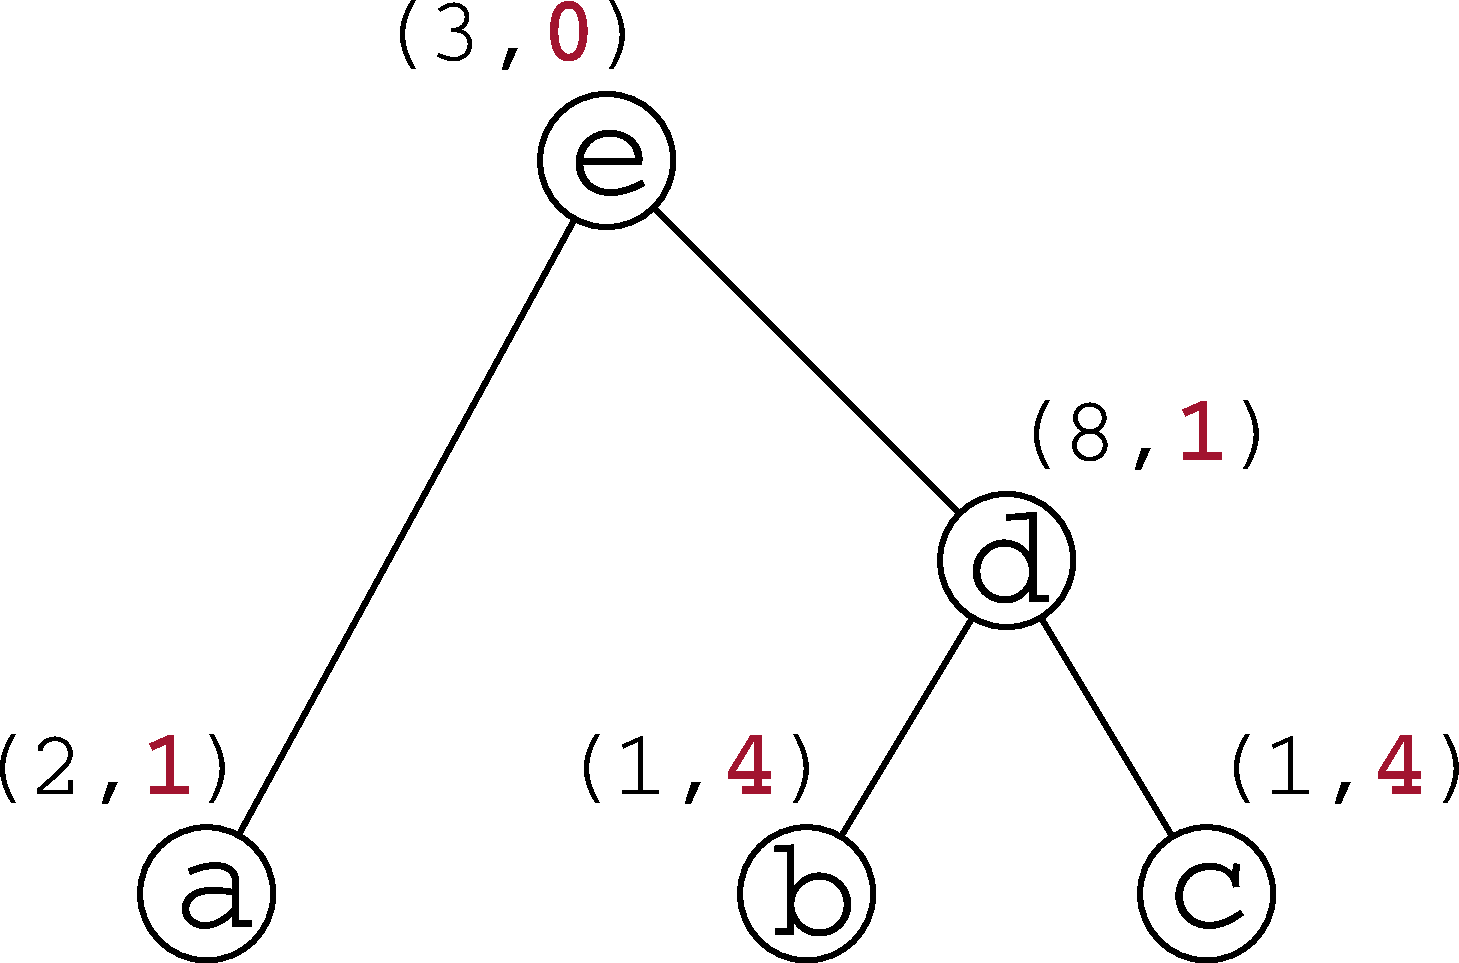
\includegraphics[width=\textwidth]{figures/memmf_cb}}%
      \only<4>{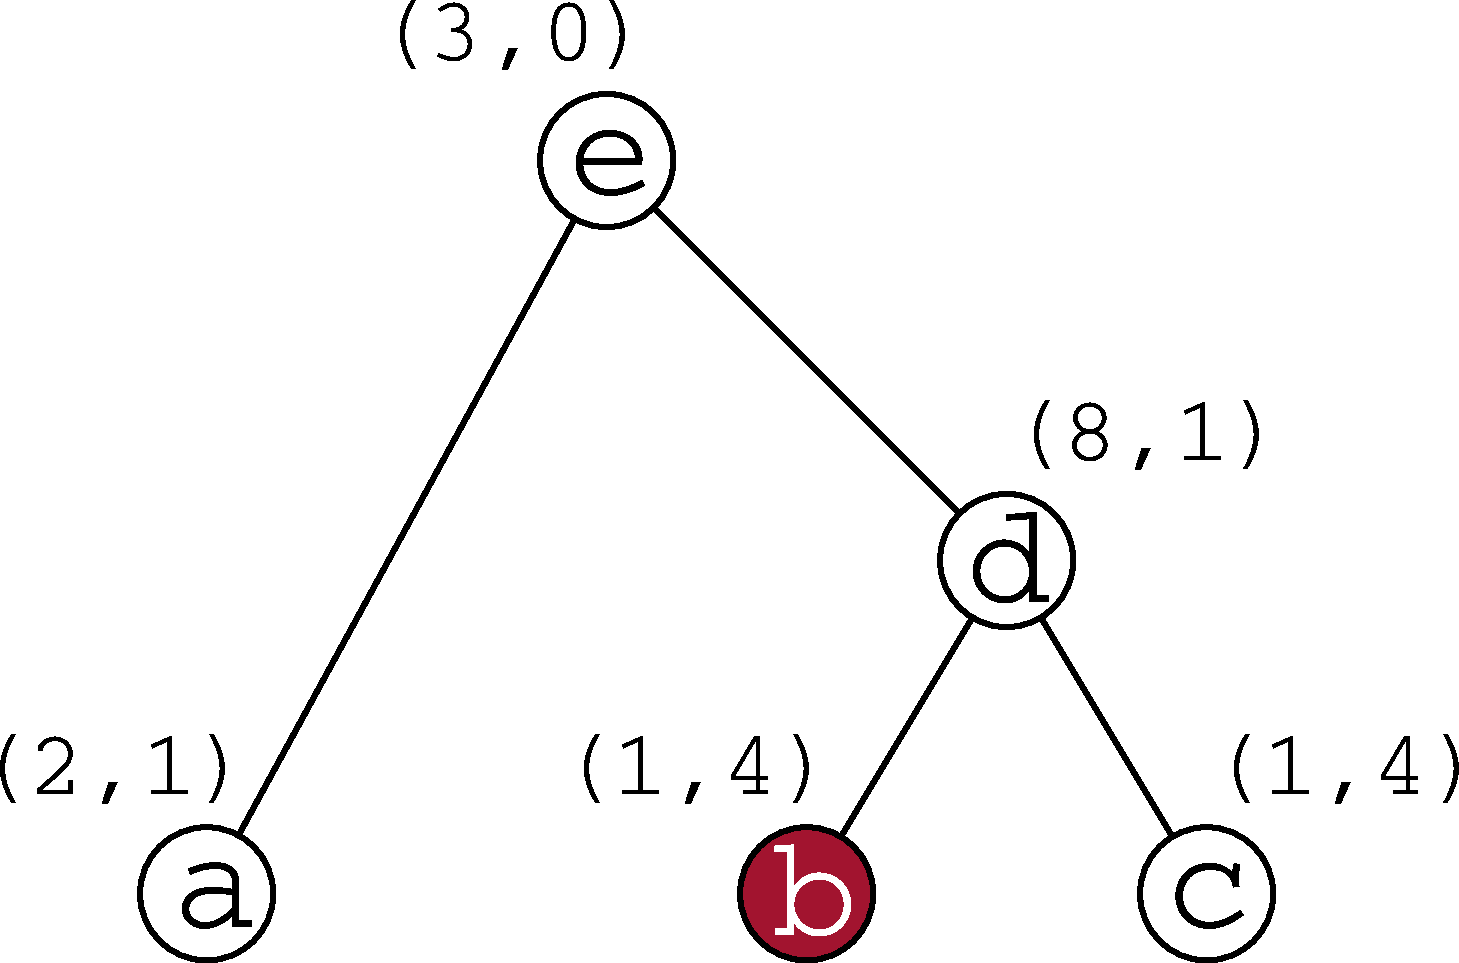
\includegraphics[width=\textwidth]{figures/memmf-opt1}}%
      \only<5>{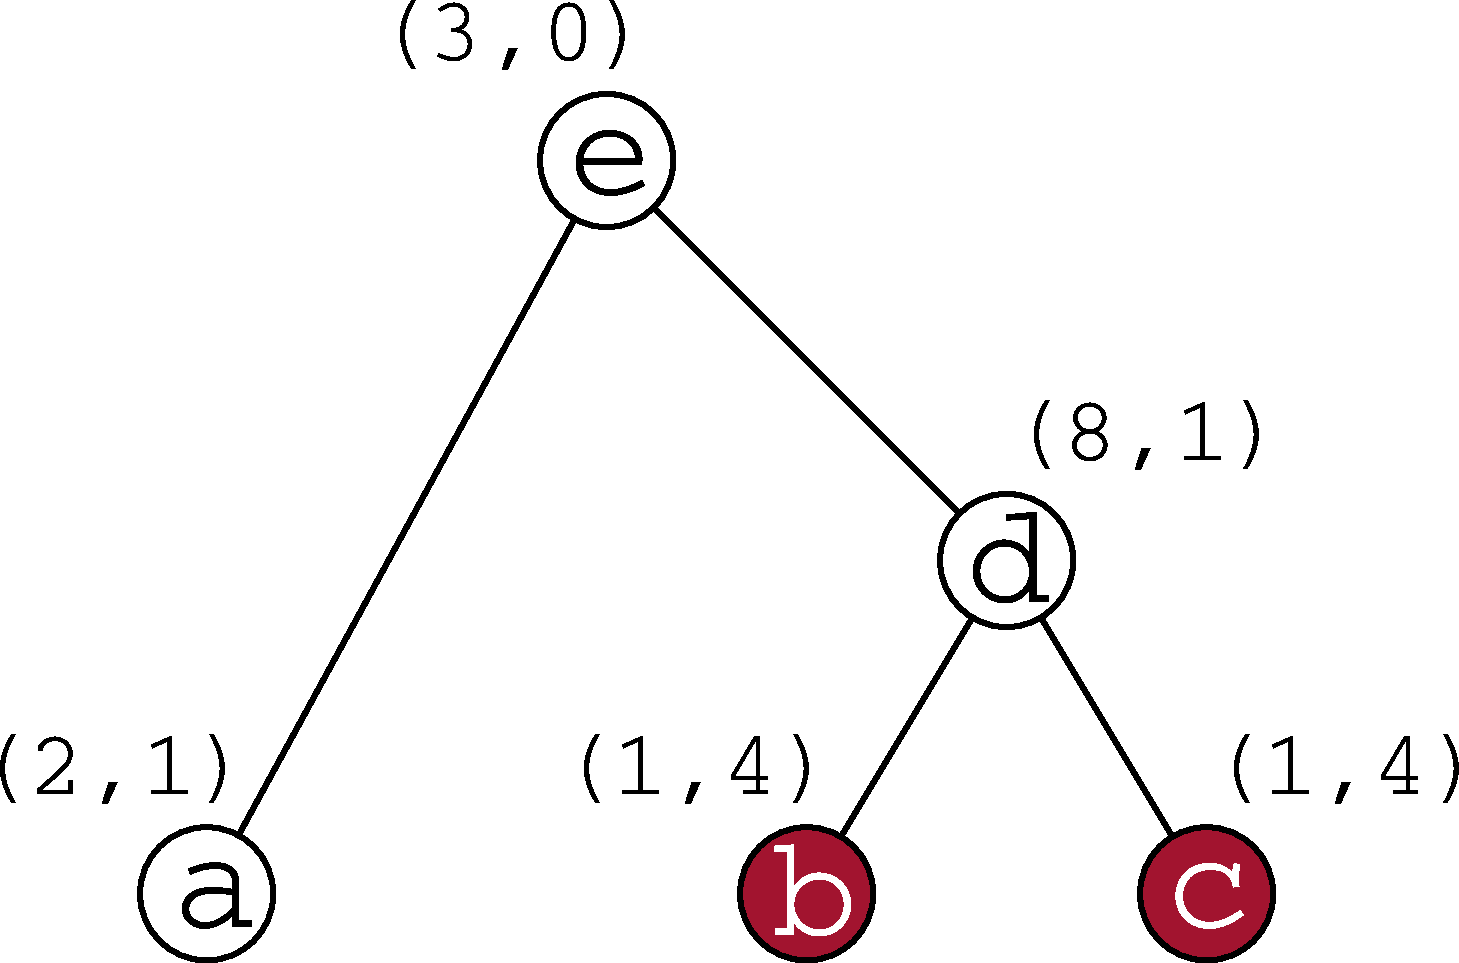
\includegraphics[width=\textwidth]{figures/memmf-opt2}}%
      \only<6>{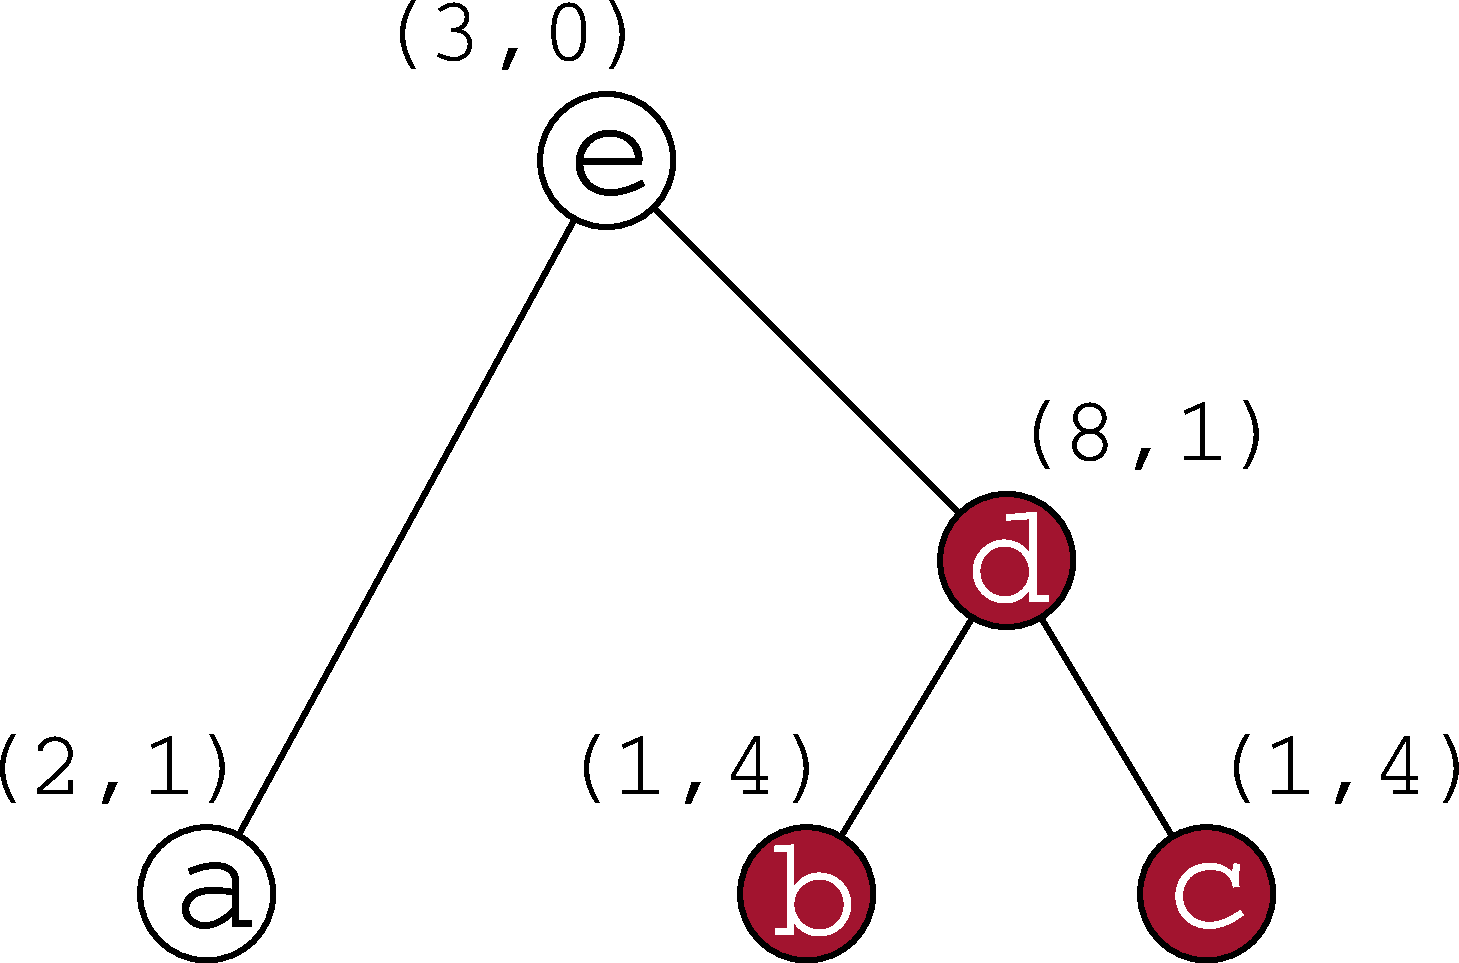
\includegraphics[width=\textwidth]{figures/memmf-opt3}}%
      \only<7>{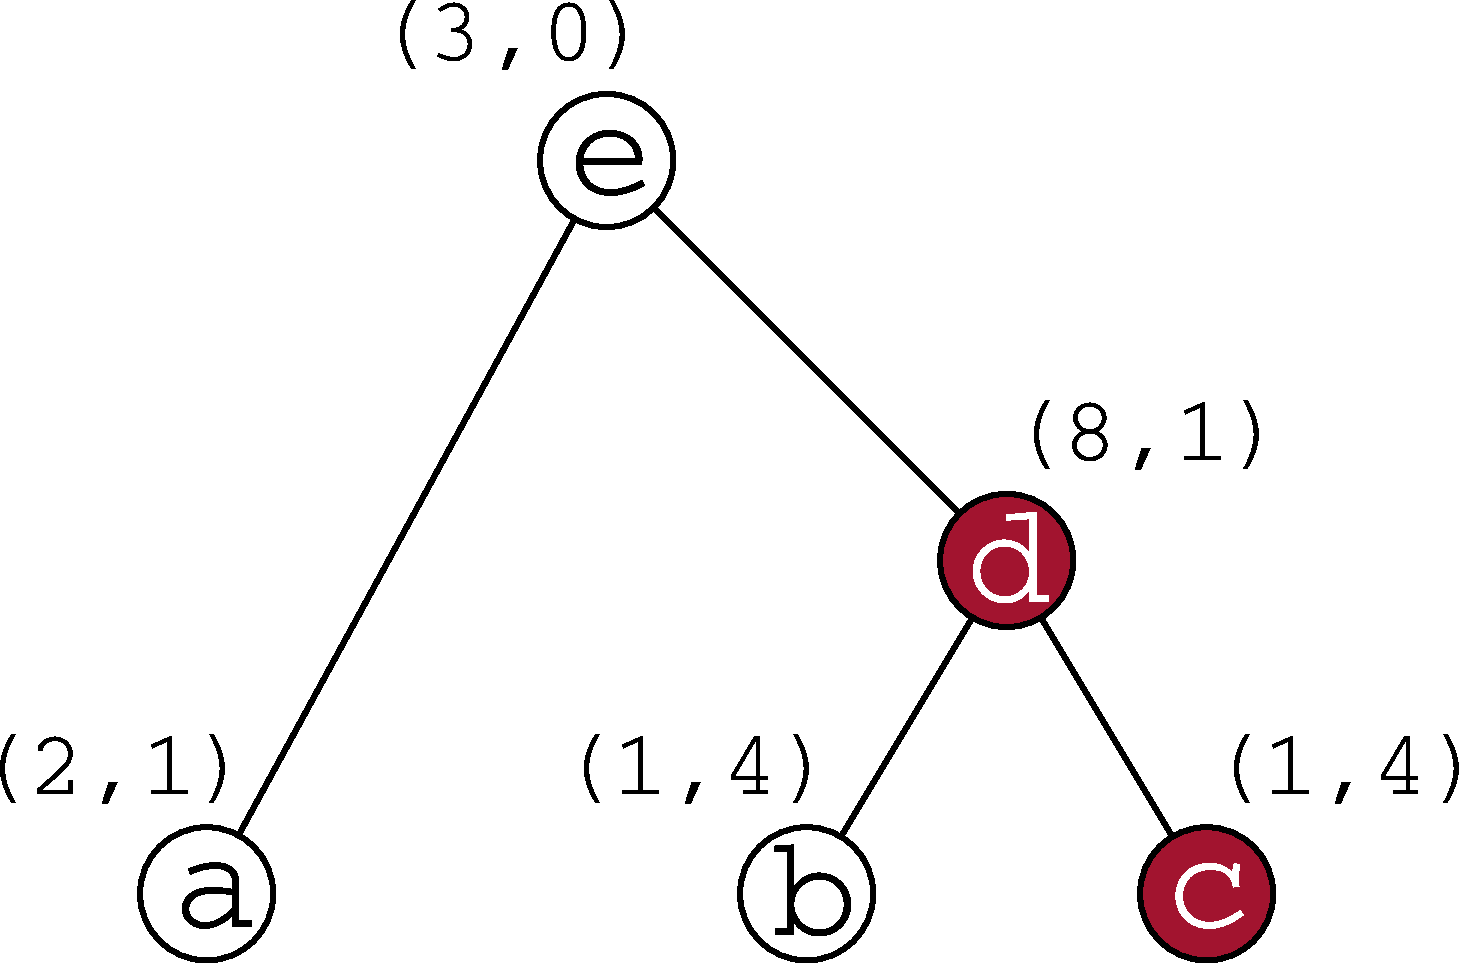
\includegraphics[width=\textwidth]{figures/memmf-opt4}}%
      \only<8>{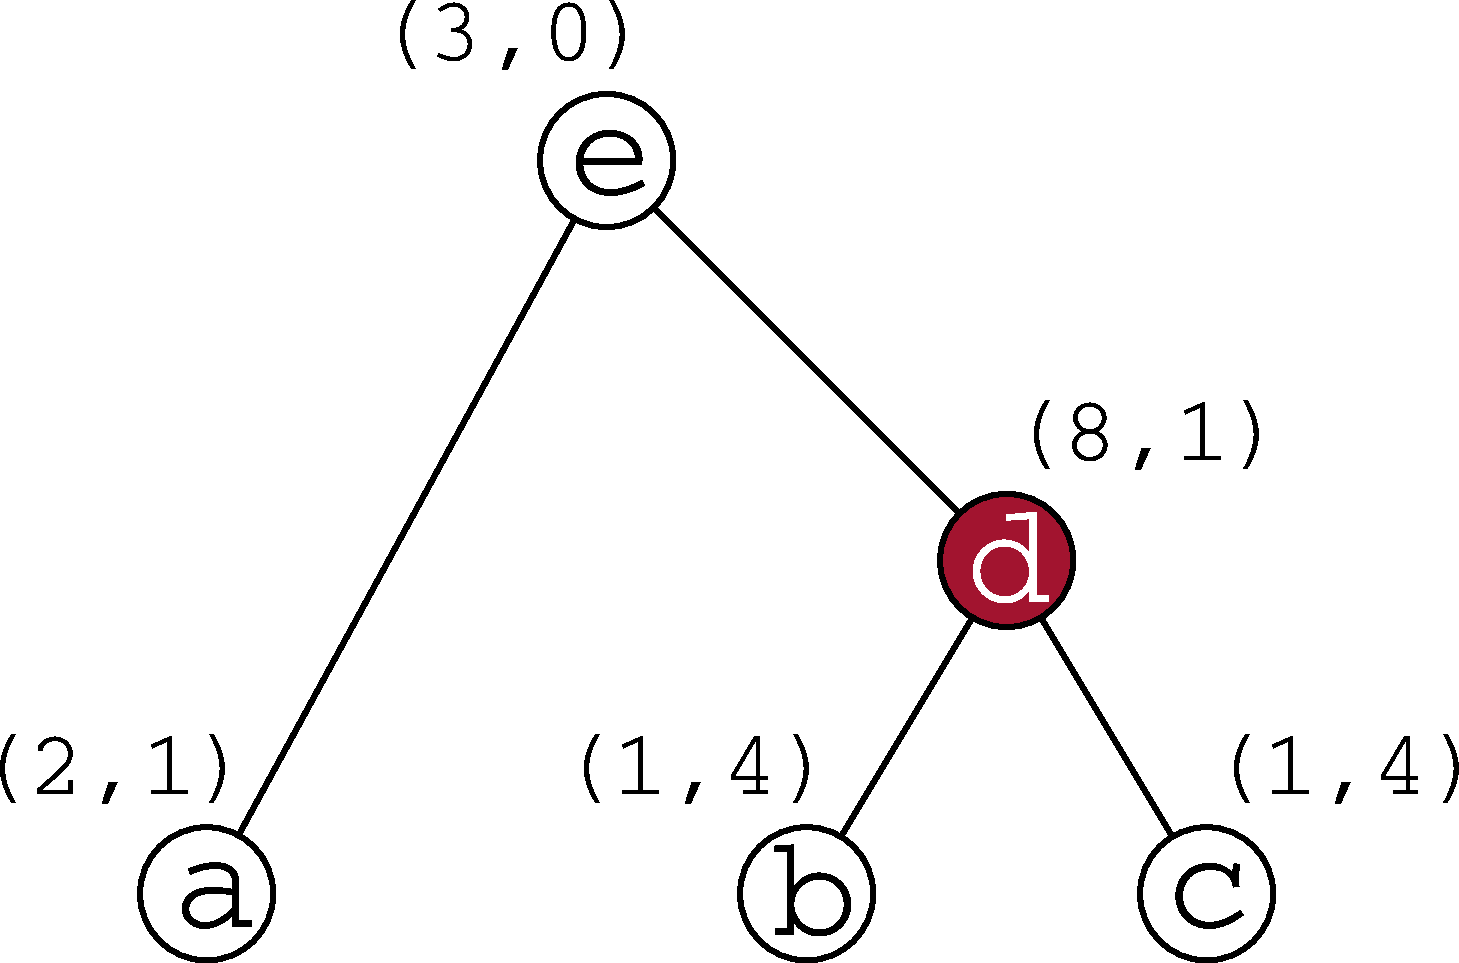
\includegraphics[width=\textwidth]{figures/memmf-opt5}}%
      \only<9>{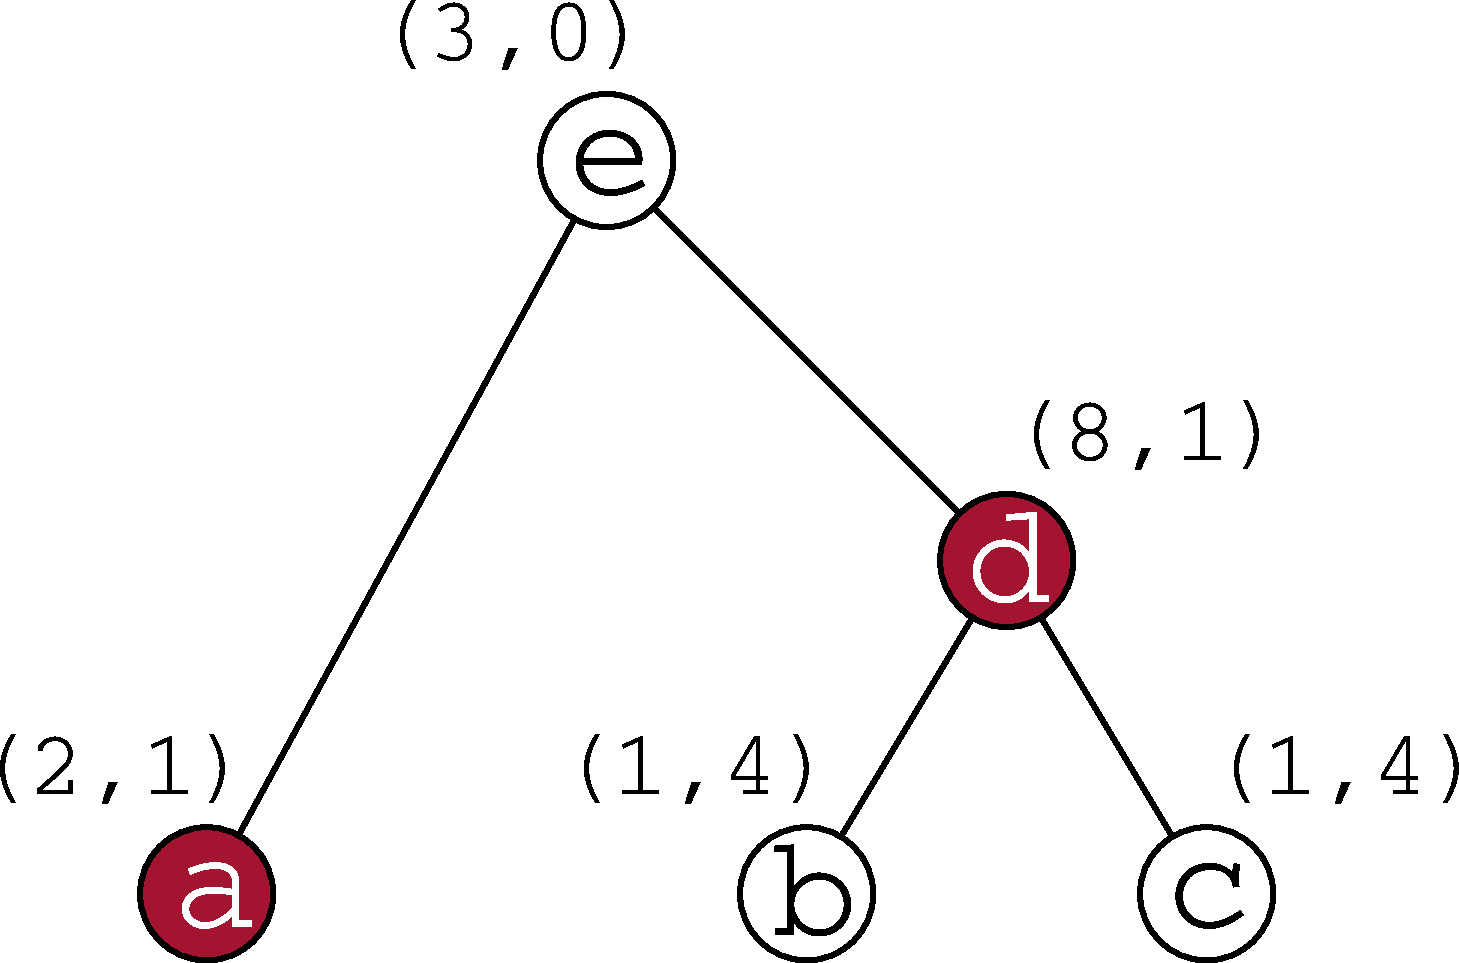
\includegraphics[width=\textwidth]{figures/memmf-opt6}}%
      \only<10>{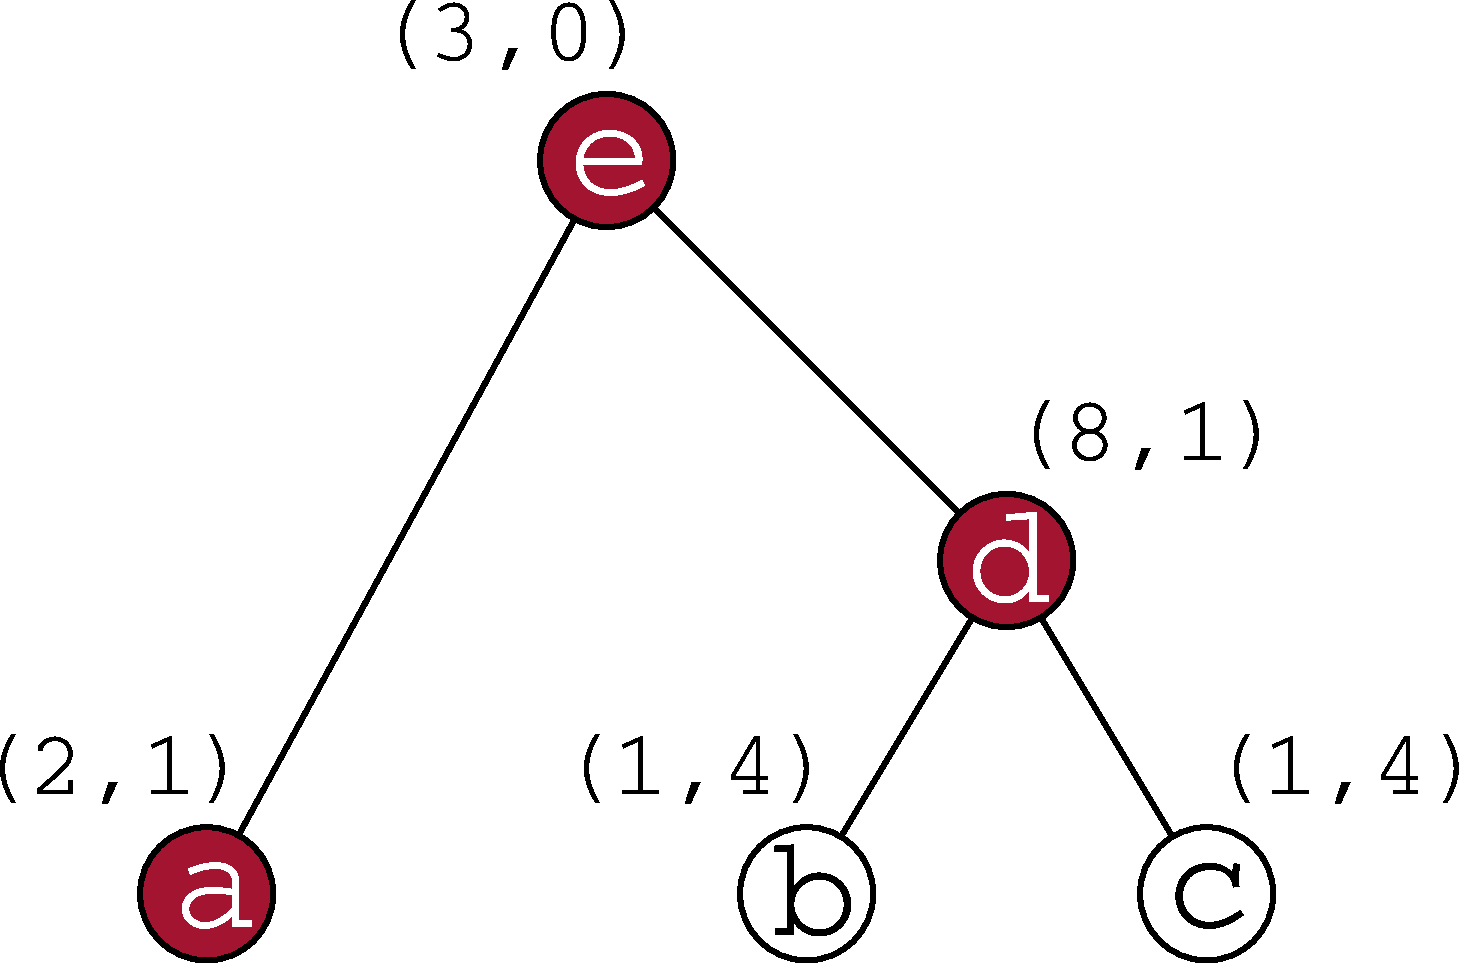
\includegraphics[width=\textwidth]{figures/memmf-opt7}}%
      \only<11>{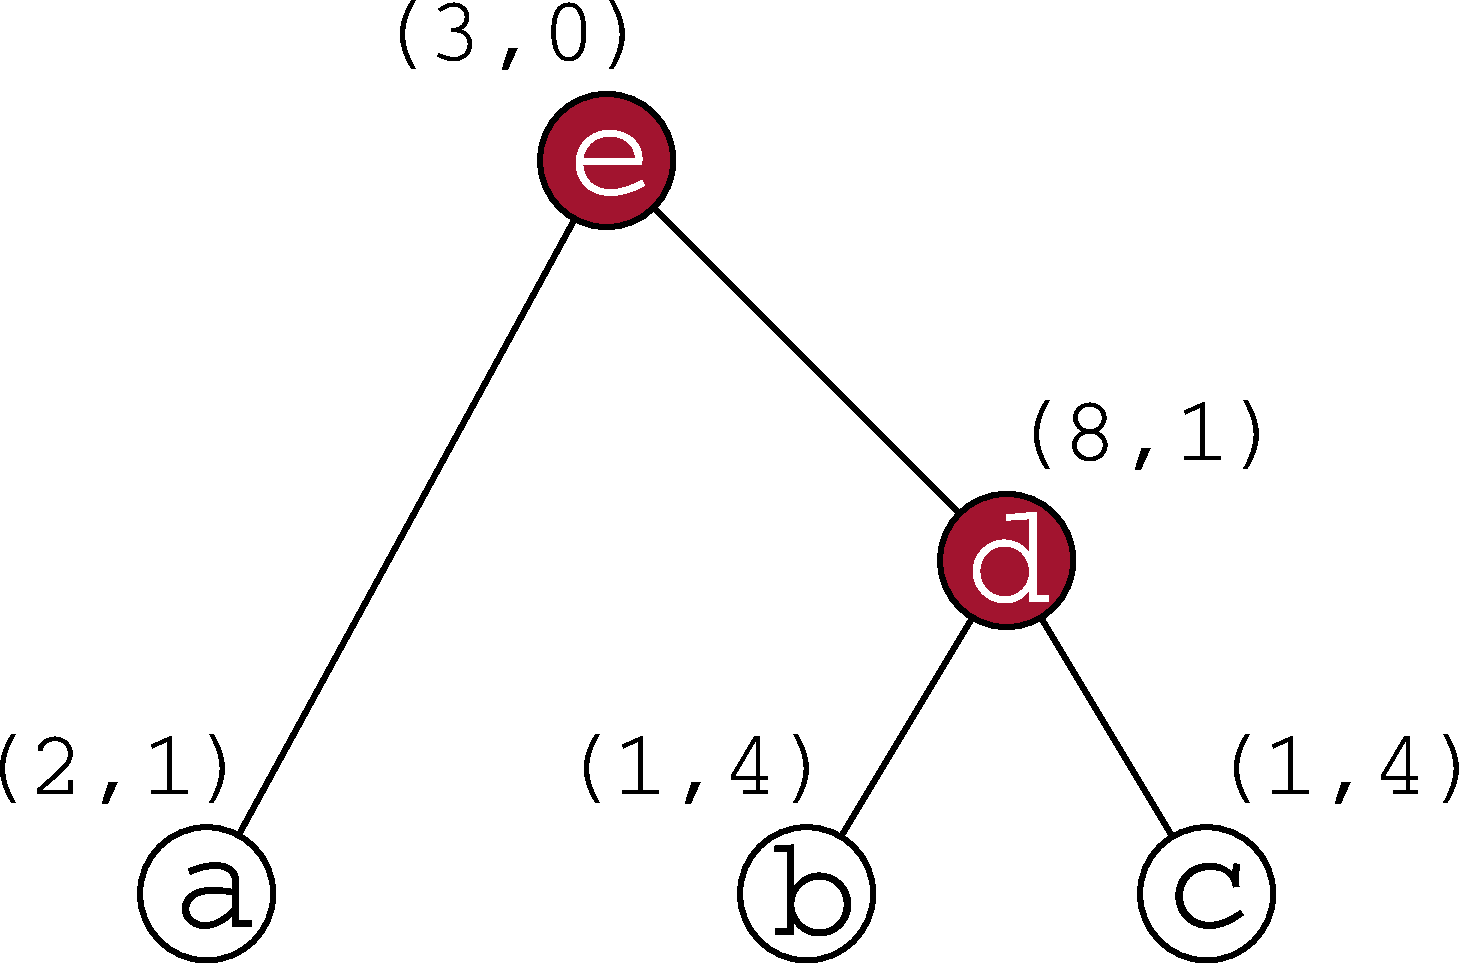
\includegraphics[width=\textwidth]{figures/memmf-opt8}}%
      \only<12->{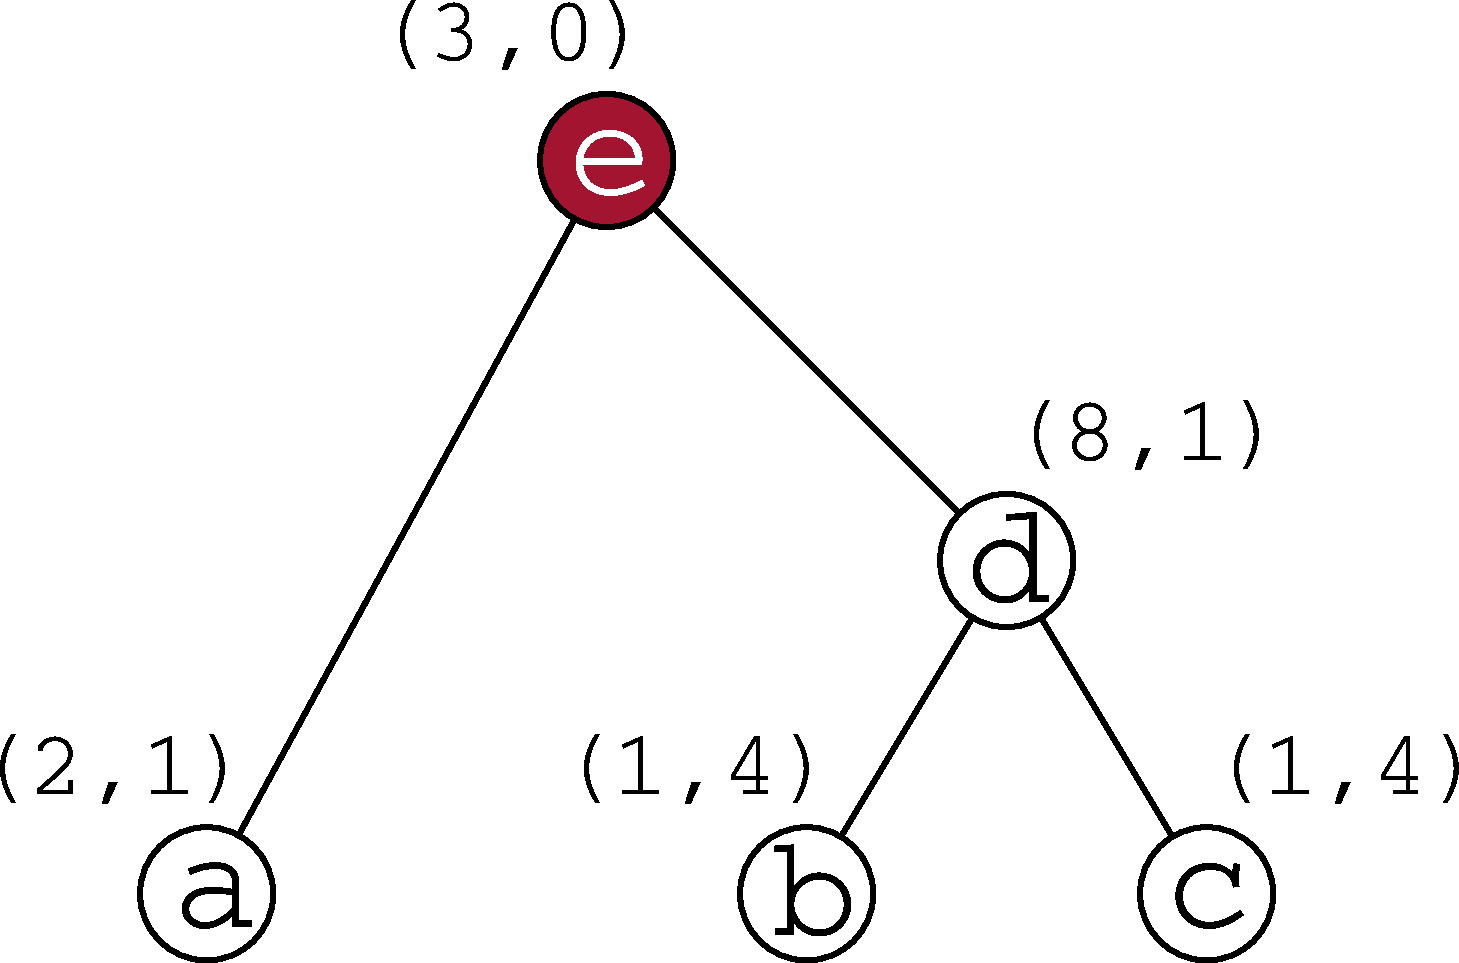
\includegraphics[width=\textwidth]{figures/memmf-opt9}}%
      
    \end{column}
    \begin{column}{0.5\textwidth}

      \begin{tabular}{r|r}
        Task & Memory \\

        \uncover<4->{\texttt{allocate(b)}}    & \uncover<4->{5}       \\
        \uncover<5->{\texttt{allocate(c)}}    & \uncover<5->{10}      \\
        \uncover<6->{\texttt{allocate(d)}}    & \uncover<6->{\dr{19}} \\
        \uncover<7->{\texttt{deallocate(b)}}  & \uncover<7->{15}      \\
        \uncover<8->{\texttt{deallocate(c)}}  & \uncover<8->{11}      \\
        \uncover<9->{\texttt{allocate(a)}}    & \uncover<9->{14}      \\
        \uncover<10->{\texttt{allocate(e)}}   & \uncover<10->{17}     \\
        \uncover<11->{\texttt{deallocate(a)}} & \uncover<11->{16}     \\
        \uncover<12->{\texttt{deallocate(d)}} & \uncover<12->{15}     \\
      \end{tabular}

    \end{column}
  \end{columns}
  
  \vspace{0.5cm}

  The memory usage varies during the factorization as the frontal
  matrices are \dr{allocated} and \dr{deallocated}. Memory usage is
  split in two:

  \begin{itemize}
    \uncover<2->{\item A \dr{persistent} memory containing the
      computed factors.}    
    \uncover<3->{\item A \dr{temporary} memory containing the
      contribution blocks, freed when a front is deallocated.}
  \end{itemize}

\end{frame}

\begin{frame}{Memory footprint in the multifrontal method}

  \begin{center}
    \only<1>{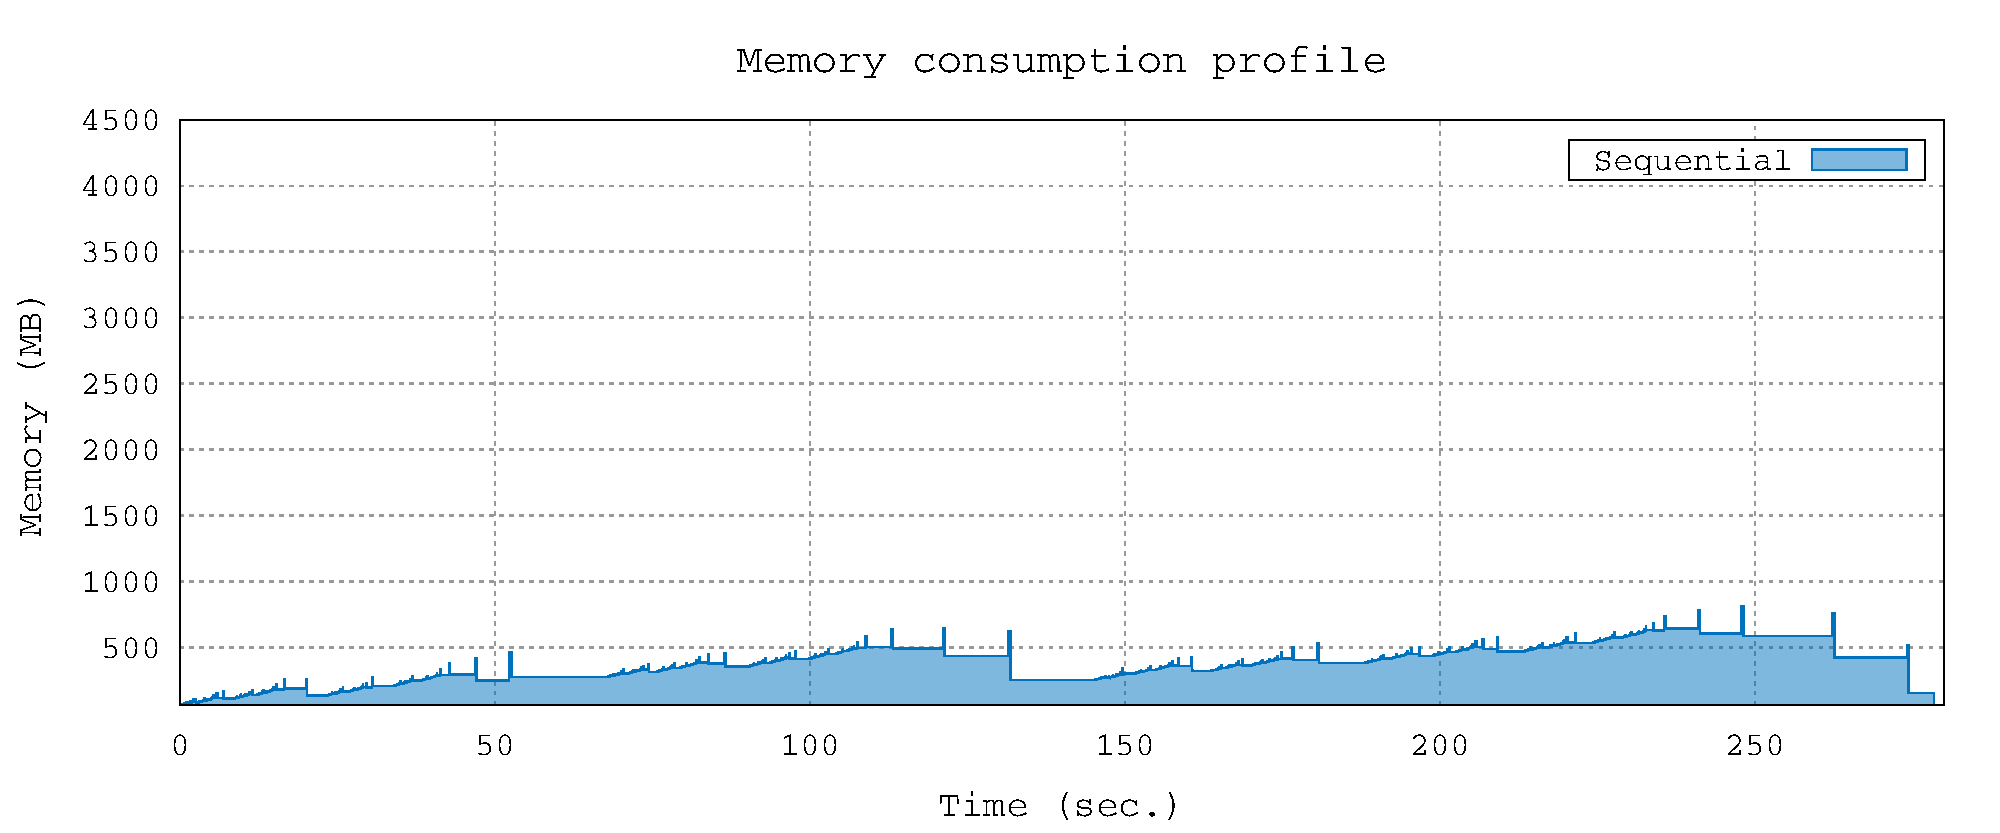
\includegraphics[width=\textwidth]{data/hirlam_ma_profile_seq}}
    \only<2->{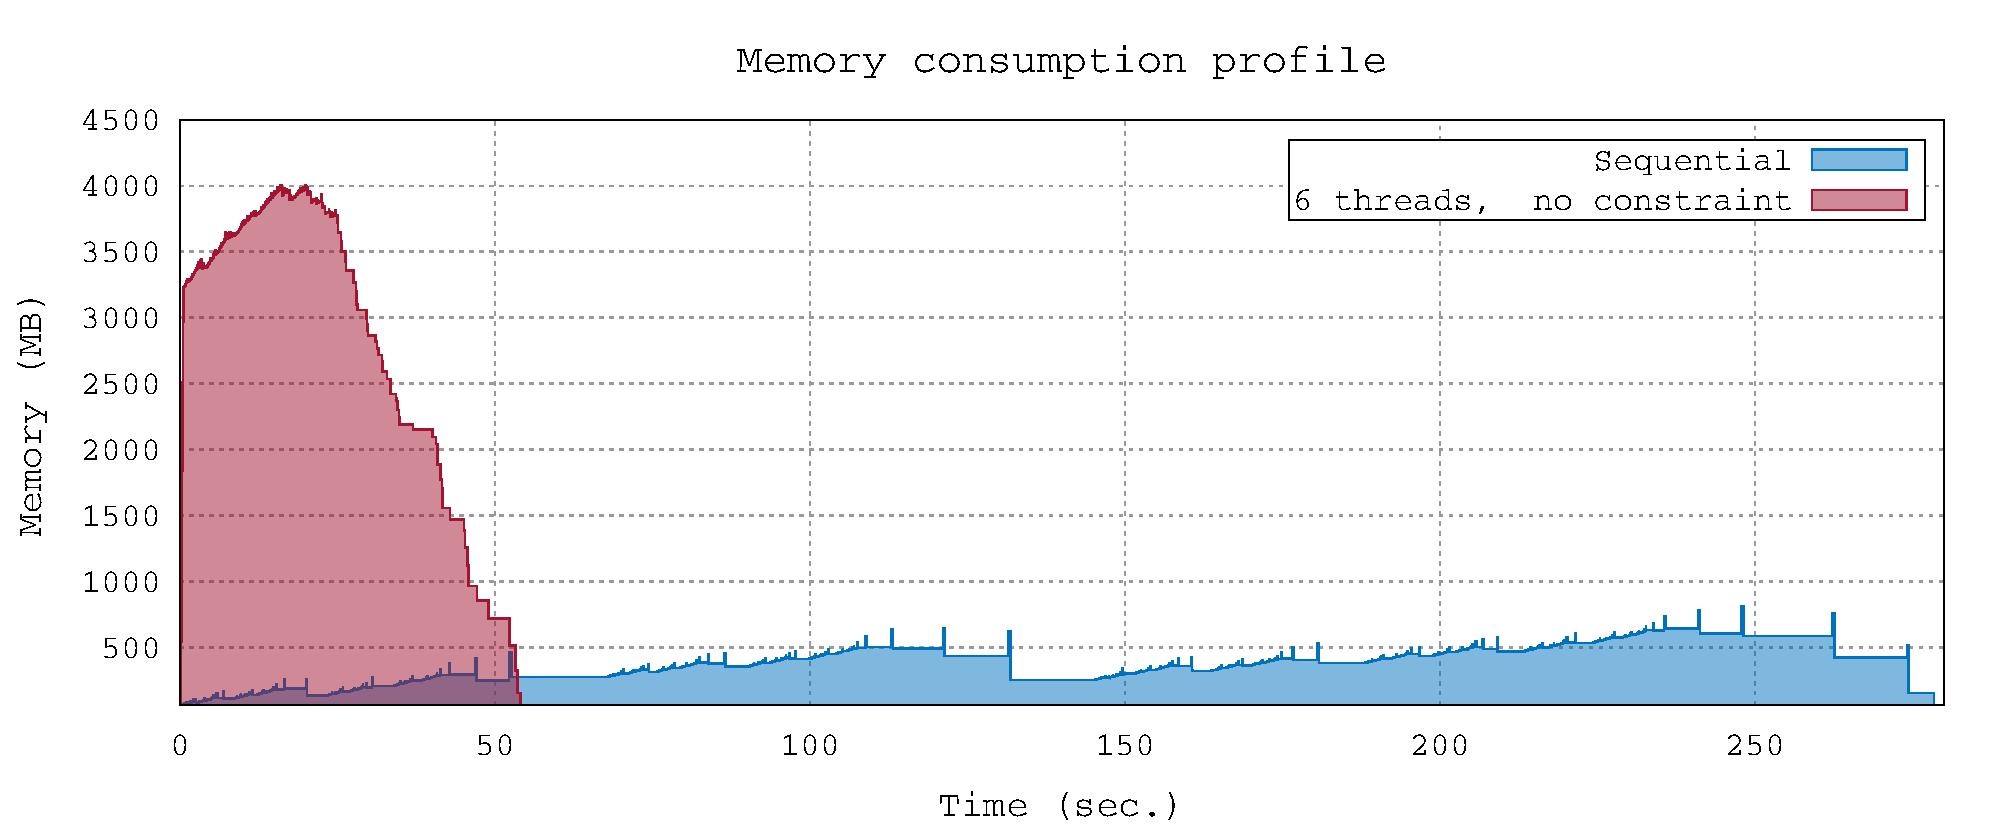
\includegraphics[width=\textwidth]{data/hirlam_ma_profile2}}
  \end{center}

  \begin{itemize}
    \uncover<2->{\item Tree-level parallelism increases the memory
      consumption.}

    \uncover<2->{\item During a parallel execution, the memory
      consumption is generally \dr{much bigger} than the sequential
      memory consumption.}
  \end{itemize}

\end{frame}

\begin{frame}{Experimental results: memory constrained factorization}

  \begin{center}
    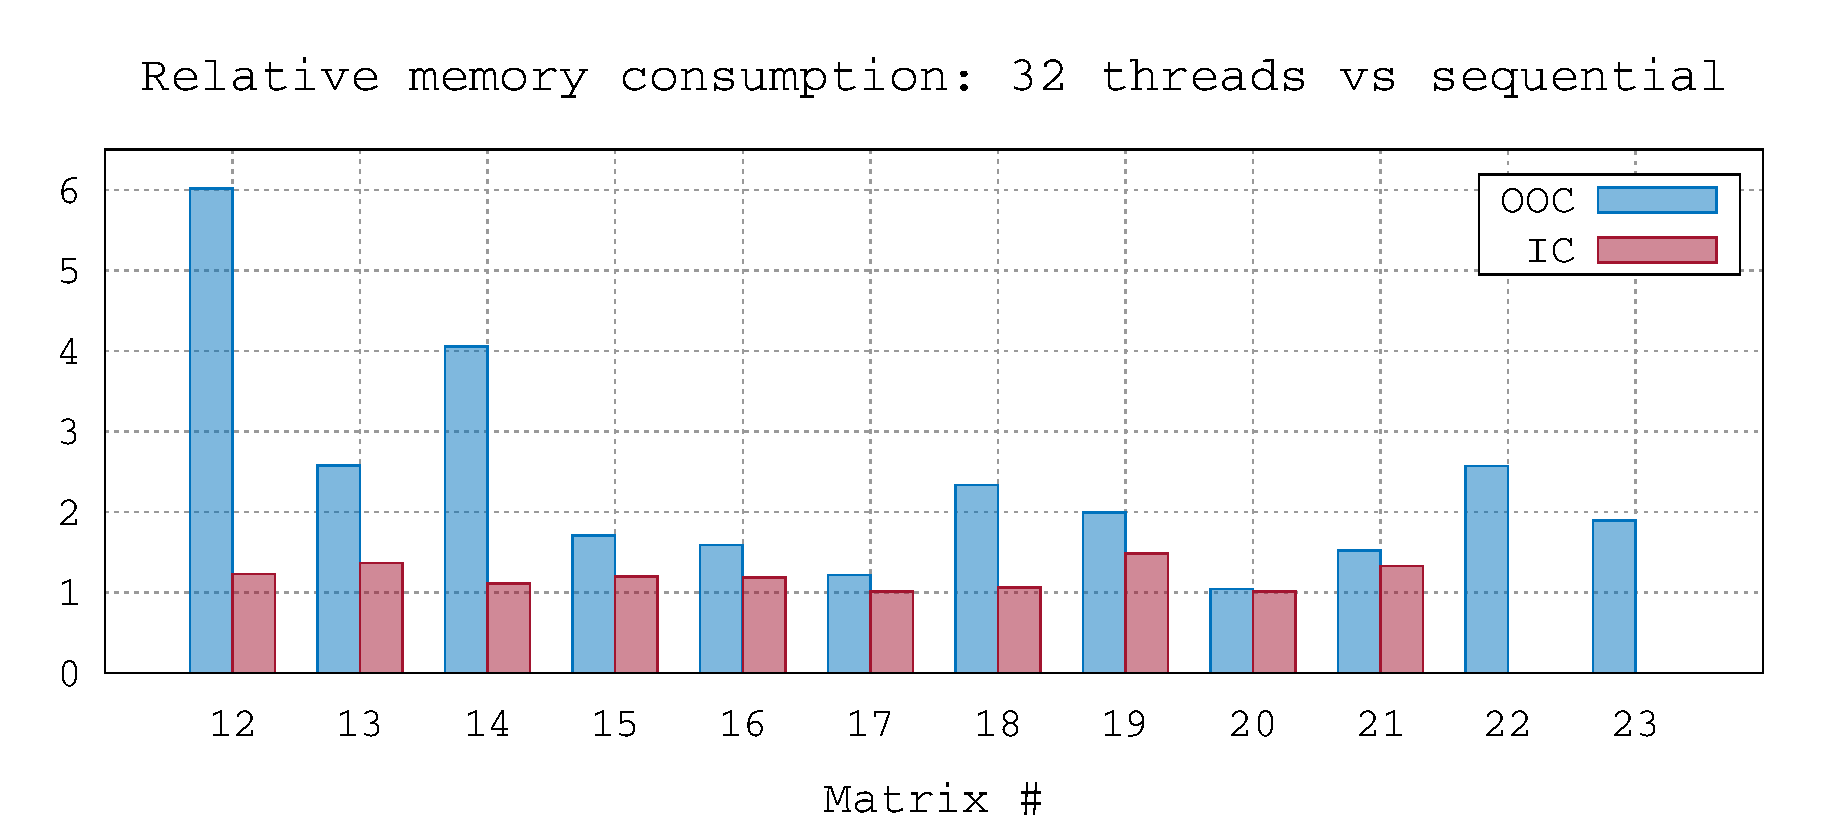
\includegraphics[width=\textwidth]{data/relative_mem2}
  \end{center}
  
  Two scenarios for the parallel execution:
  \begin{itemize}
  \item In-Core (IC) execution: this is the most common case where the
    computed factors are kept in memory.
  \item Out-Of-Core (OOC) execution: in this scenario the factors are
    written to disk as they are computed in order to save memory.
  \end{itemize}

\end{frame}

\begin{frame}{Task scheduling under memory constraint}

  \vspace{-1cm}

  \begin{block}{Memory-aware parallel execution}
    \alert{Objective}: achieve efficient parallel execution within a
    prescribed memory consumption
    \alert{$M_p \le \alpha M_s,~~\alpha \ge 1$}.
  \end{block}

  \uncover<2->{
    
    \vspace{0.3cm}
    
    \alert{Method}: suspend tasks submission when no more memory is
    available and resume it when enough memory has been freed by
    previously submitted tasks.}
  
    \vspace{0.3cm}
  
    \begin{columns}
      \begin{column}{0.5\textwidth}

        % \vspace{0.2cm}

        \uncover<3->{Special care must be taken to avoid \alert{memory
            deadlocks}.}

        \vspace{0.2cm}

        \uncover<4>{Example: if $M_p=1.0 M_s=19$ memory units, concurrent
        allocation of fronts \texttt{a}, \texttt{b} and \texttt{c}
        will result in a deadlock.}
      \end{column}
      \begin{column}{0.5\textwidth}
        \begin{overlayarea}{\textwidth}{2cm}
          \begin{center}
            \only<3>{\includegraphics[width=\textwidth]{figures/memmf}}%
            \only<4>{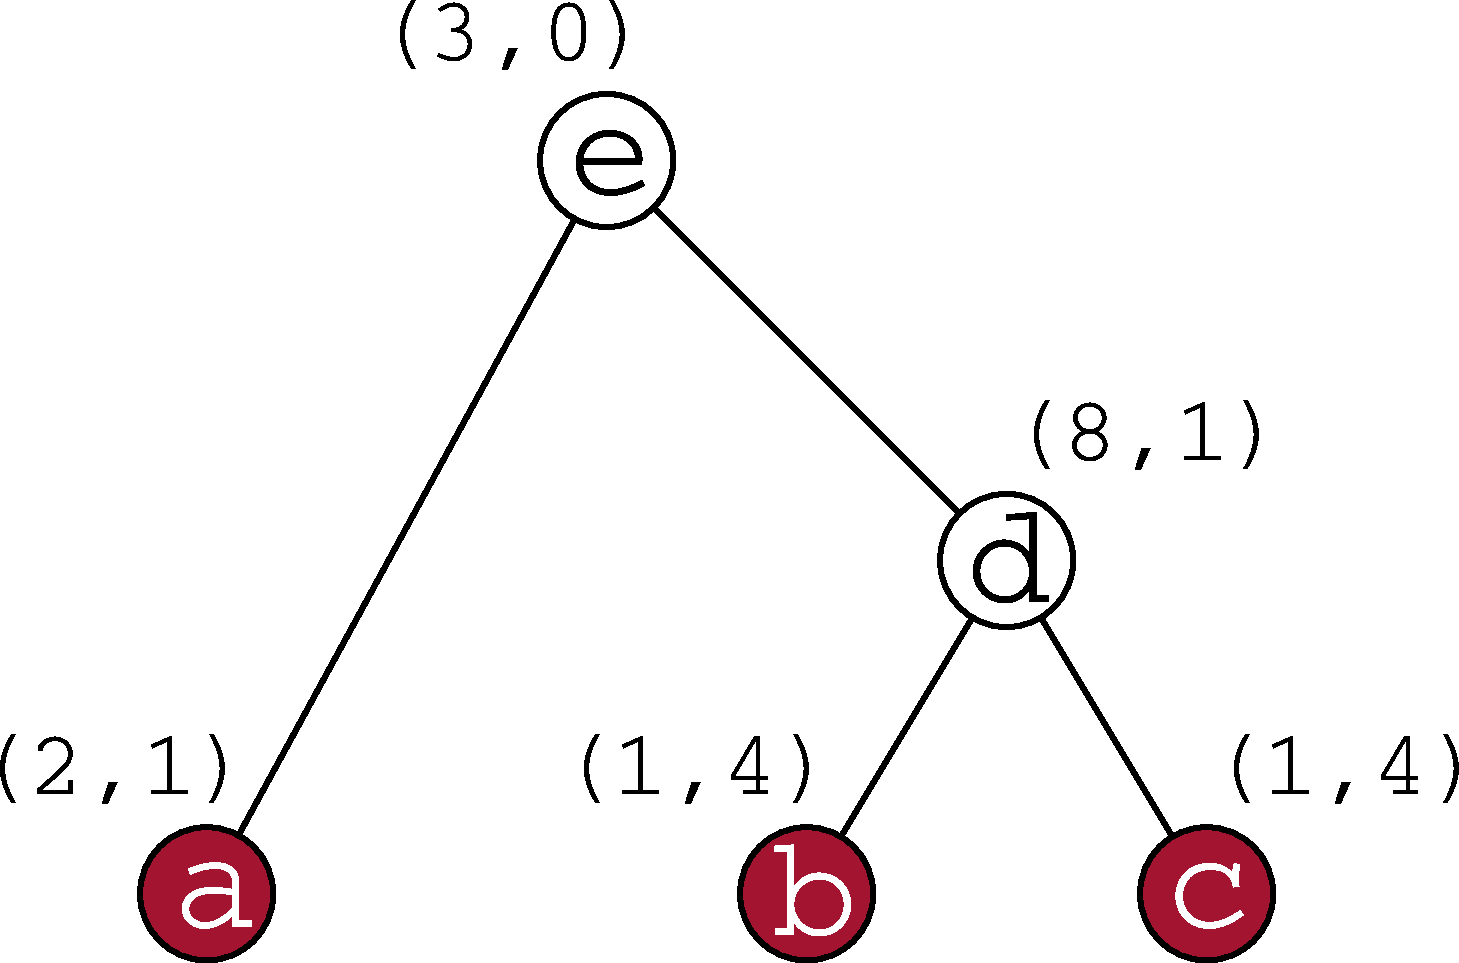
\includegraphics[width=\textwidth]{figures/memmf_par}}%
          \end{center}
        \end{overlayarea}
      \end{column}
    \end{columns}
\end{frame}

\begin{frame}{Task scheduling under memory constraint}

  \begin{block}{Deadlock prevention}
    Organize resource (memory) usage by each process to ensure that at
    least one process is always able to get all the resources it
    needs (Agullo \textit{et al.}, Marchal \textit{et al.}, Amestoy \textit{et al.}).
  \end{block}

  \uncover<2->{\alert{Approach}: the allocation of fronts is forced to
  respect the \alert{sequential order}. }
  % The tasks
  % submitted as a results of a front allocation can be executed in
  % any order.}
  
  \vspace{-0.2cm}
  
  \begin{overlayarea}{\textwidth}{4cm}
    \begin{center}
      \only<2>{\includegraphics[width=0.5\textwidth]{figures/memmf}}%
      \only<3>{\includegraphics[width=0.5\textwidth]{figures/memmf_act}}
    \end{center}
  \end{overlayarea}

  \uncover<3>{This ensures that the parallel execution can run to completion
  within the same memory envelop as the sequential one.}


\end{frame}

\begin{frame}[fragile,t,plain]{Memory aware scheduling in a STF model}

\begin{lstlisting}[basicstyle=\tt\tiny]
do f=1, nfronts ! in postorder

   call activate(f)    ! compute structure and register handles

   call submit(init, f) ! allocate and initialize front

   do c=1, f%nc ! for all the children of f
      do j=1,c%n
         ! assemble column j of c into f
         call submit(assemble, c, j, f)
      end do
      ! cleanup child
      call submit(clean, c)
   end do

   do p=1, f%n
      ! panel reduction of column p
      call submit(_geqrt, f, p)
      do u=p+1, f%n
         ! update of column u with panel p
         call submit(_gemqrt, f, u, p)
      end do
   end do
end do
! wait for the tasks to be executed
call wait_tasks_completion()
\end{lstlisting}
\end{frame}

\begin{frame}[fragile,t,plain]{Memory aware scheduling in a STF model}
\begin{lstlisting}[basicstyle=\tt\tiny]
do f=1, nfronts ! in postorder
   do while(avail_mem < size(f)) wait()
   
   call allocate(f)    ! allocate front: avail_mem -= size (f)

   call activate(f) ! compute structure and register handles
   
   call submit(init, f) ! initialize front

   do c=1, f%nc ! for all the children of f
      do j=1,c%n
         ! assemble column j of c into f
         call submit(assemble, c, j, f)
      end do
      ! cleanup child: avail_mem += size ( cb ( f ) )
      call submit(clean, c)
   end do

   do p=1, f%n
      ! panel reduction of column p
      call submit(_geqrt, f, p)
      do u=p+1, f%n
         ! update of column u with panel p
         call submit(_gemqrt, f, u, p)
      end do
   end do
end do
! wait for the tasks to be executed
call wait_tasks_completion()
\end{lstlisting}

\end{frame}

% \begin{frame}{Experimental results: memory constrained factorization}
%   \centering
%   \includegraphics[width=\textwidth]{ma_times_1d}
% \end{frame}

\begin{frame}{Experimental results: memory constrained factorization}
  \centering
  \alert{$M_p \le \alpha M_s,~~\alpha=\{1.0,1.2,1.4,1.6,1.8,2.0\}$}
  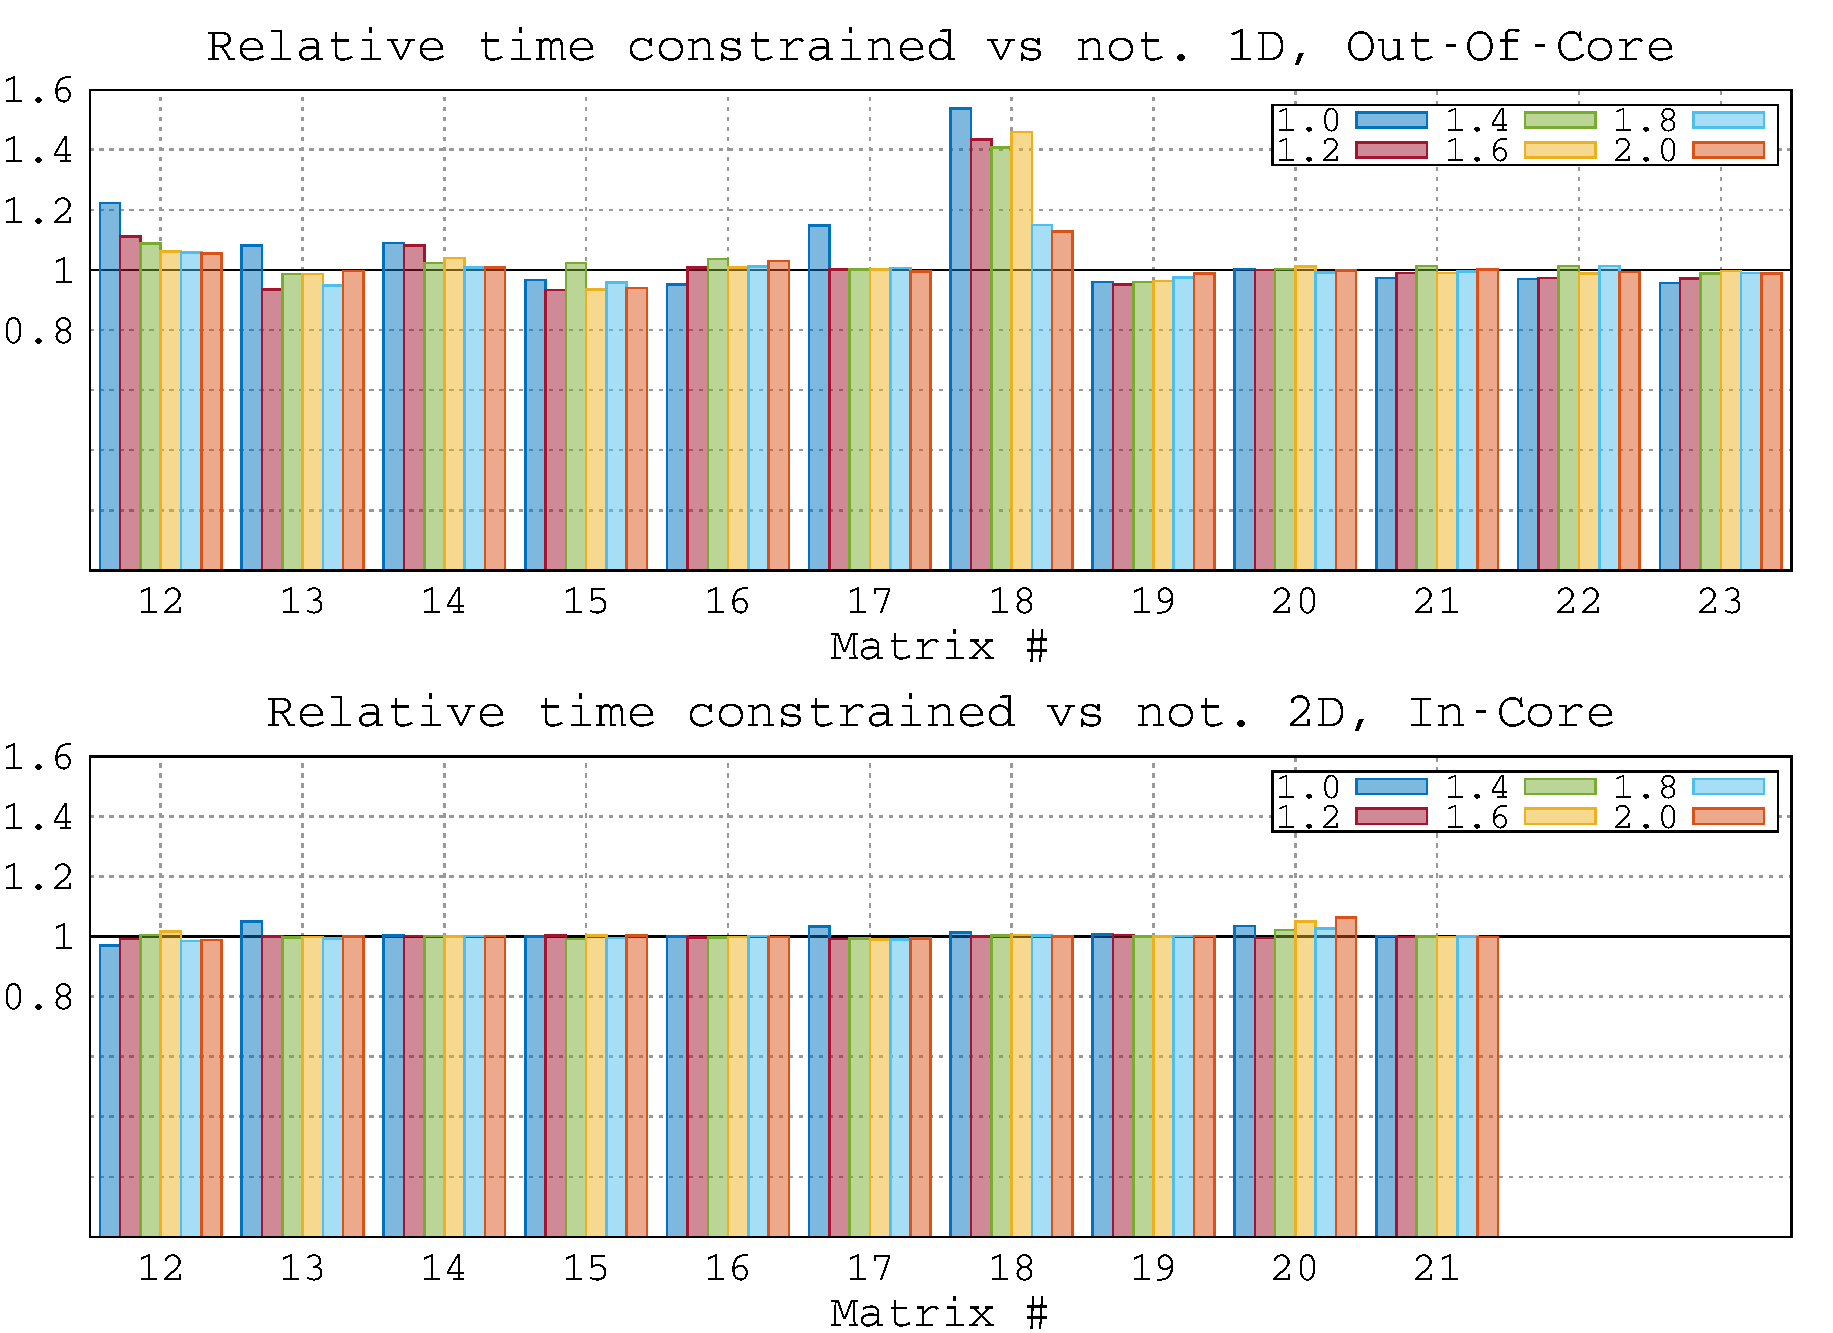
\includegraphics[width=0.95\textwidth]{data/ma_times2}
\end{frame}

% \begin{frame}{Task scheduling under memory constraint}

%   \dr{Problem}: minimize the memory footprint of the factorization.
   
%   \db{Sequential} case:
%   \begin{itemize}
%   \item Memory-minimizing postorder traversal: Liu's
%     algorithms~\cite{l:86}
%   \end{itemize}

%   \db{Parallel} case:
%   \begin{itemize}
%   \item The problem is \dr{NP-complete} and no \dr{approximation
%       algorithms} can be designed to tackle the
%     problem~\cite{e.m.s.v:15}.

%   \item \citet{e.m.s.v:15} propose several \dr{heuristics} such as
%     {\sc MemBookingInnerFirst} for the scheduling of task trees under
%     a given memory constraint.
%   \end{itemize}

% \end{frame}

% \begin{frame}{Task scheduling under memory constraint}

%   \dr{Objective}: limit the memory footprint of the parallel
%   factorization.  

%   \begin{overlayarea}{\textwidth}{1.5cm}    
%     \only<2-3>{\dr{Example}: Memory constraint: 19 memory units. }%
%     \only<3>{Let's assume that nodes \db{a}, \db{b} and \db{c} are
%       activated in parallel consuming 13 meory units and node \db{d}
%       cannot be allocated: \alert{Deadlock}.}

%     \only<4->{\dr{Approach}: the activation of fronts is forced to
%       respect the memory-minimizing sequential order. The tasks
%       submitted as a results of a front activation can be executed in
%       any order.}
%   \end{overlayarea}    

%   \begin{center}
%     \only<1-2>{\includegraphics[width=0.5\textwidth]{memmf}}%
%     \only<3>{\includegraphics[width=0.5\textwidth]{memmf3}}%
%     \only<4->{\includegraphics[width=0.5\textwidth]{memmf_act}}%
%   \end{center}  

%   \uncover<5->{This ensures that the parallel execution runs within
%     the same memory envelop as the sequential one. The memory
%     constraint can be relaxed in order to permit the activation of
%     more fronts and, potentially achieve more concurrency.}

% \end{frame}

% \begin{frame}[fragile,t,plain]{Memory aware scheduling in a STF model}

% \begin{lstlisting}[basicstyle=\tt\tiny]
% do f=1, nfronts ! in postorder

%    call activate(f)    ! compute structure and register handles

%    call submit(init, f) ! allocate and initialize front

%    do c=1, f%nc ! for all the children of f
%       do j=1,c%n
%          ! assemble column j of c into f
%          call submit(assemble, c, j, f)
%       end do
%       ! cleanup child
%       call submit(clean, c)
%    end do

%    do p=1, f%n
%       ! panel reduction of column p
%       call submit(panel, f, p)
%       do u=p+1, f%n
%          ! update of column u with panel p
%          call submit(update, f, u, p)
%       end do
%    end do
% end do
% ! wait for the tasks to be executed
% call wait_tasks_completion()
% \end{lstlisting}
% \end{frame}

% \begin{frame}[fragile,t,plain]{Memory aware scheduling in a STF model}
% \begin{lstlisting}[basicstyle=\tt\tiny]
% do f=1, nfronts ! in postorder
%    do while(avail_mem < size(f)) wait()

%    call activate(f) ! compute structure and register handles
   
%    call allocate(f)    ! allocate front: avail_mem -= size (f)

%    call submit(init, f) ! initialize front

%    do c=1, f%nc ! for all the children of f
%       do j=1,c%n
%          ! assemble column j of c into f
%          call submit(assemble, c, j, f)
%       end do
%       ! cleanup child: avail_mem += size ( cb ( f ) )
%       call submit(clean, c)
%    end do

%    do p=1, f%n
%       ! panel reduction of column p
%       call submit(panel, f, p)
%       do u=p+1, f%n
%          ! update of column u with panel p
%          call submit(update, f, u, p)
%       end do
%    end do
% end do
% ! wait for the tasks to be executed
% call wait_tasks_completion()
% \end{lstlisting}

% \end{frame}

% \begin{frame}{Experimental results: memory constrained factorization}
%   \begin{center}
%     \includegraphics[width=\textwidth]{relative_mem}
%   \end{center}
  
%   Two scenarios for the parallel execution:
%   \begin{itemize}
%   \item In-Core (IC) execution: this is the most common case where the
%     computed factors are kept in memory.
%   \item Out-Of-Core (OOC) execution: in this scenario the factors are
%     written to disk as they are computed in order to save memory.
%   \end{itemize}

% \end{frame}

% % \begin{frame}{Experimental results: memory constrained factorization}
% %   \centering
% %   \includegraphics[width=\textwidth]{ma_times_1d}
% % \end{frame}

% \begin{frame}{Experimental results: memory constrained factorization}
%   \centering
%   \includegraphics[width=\textwidth]{ma_times_2d}
% \end{frame}

%%% Local Variables:
%%% mode: latex
%%% TeX-master: "defense"
%%% TeX-engine: xetex
%%% End:
